\section{Assignment 1: Colorizing Images}
\label{sec:assignment1}

The goal of this assignment is to assemble a colorized image given three color channel images. As the three channels are not perfectly aligned the program has to also align them automatically.


\subsection{Methodology}

For the above purpose, we use normalized cross-correlation as the matching metric. The return value of the metric for each displacement (-OFFSET:OFFSET) is saved and the best displacement is used to create the final image.

In the initial version, we compare the values of R (red) channel as the base with G (green) and B (blue) channels. The best displacement of G and B compared to R are used in the final image.

In a second version, first the best displacement for G channel against R channel is determined. Then we compare various B channel displacements against R+G2 (G2 is the best displacement of green channel found in the previous step). The blue channel displacement with the best score sum is used in the final image.
The results were fairly equal in both cases, however the second experiment appears to deliver a better alignment slightly.

The algorithm does not always deliver perfectly matching images, as illustrated by Figure \ref{fig:a1:imperfect}.

\begin{figure}[h]
	\centering
	\begin{tabular}{cc}
	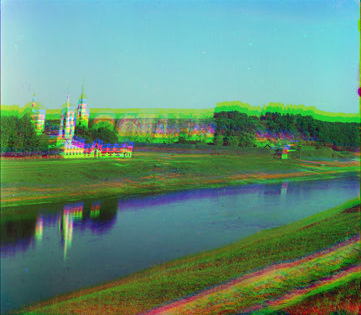
\includegraphics[width=0.48\textwidth]{figures/00125_base.png} &
	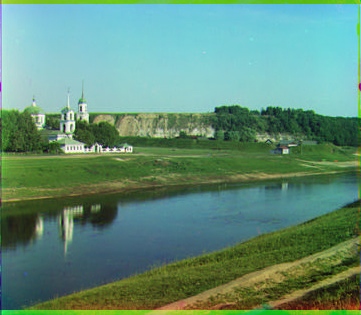
\includegraphics[width=0.48\textwidth]{figures/00125_v2.png} 

	\end{tabular}
	\caption{Base unmodified image and the final result. }
	\label{fig:a1:alignment}
\end{figure}

\begin{figure}[h]
	\centering
	\begin{tabular}{cc}
	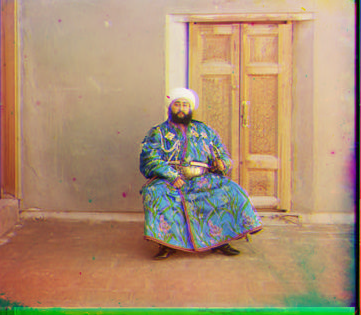
\includegraphics[width=0.48\textwidth]{figures/00153_v1.png} &
	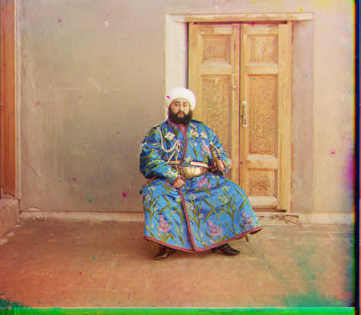
\includegraphics[width=0.48\textwidth]{figures/00153_v2.png} 

	\end{tabular}
	\caption{Largest difference between first (left) and second methods. The better displacement of blue channel is clearly recognizable. }
	\label{fig:a1:difference_v1_v2}
\end{figure}

\begin{figure}[h]
	\centering
	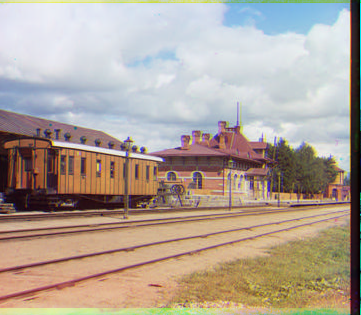
\includegraphics[width=0.48\textwidth]{figures/00398_v2.png} 

	\caption{Green channel is obviously not perfectly aligned, as visible around the outside of the trees. }
	\label{fig:a1:imperfect}
\end{figure}




